% Created 2020-10-26 Mon 16:38
% Intended LaTeX compiler: pdflatex
\documentclass[11pt]{article}
\usepackage[utf8]{inputenc}
\usepackage[T1]{fontenc}
\usepackage{graphicx}
\usepackage{grffile}
\usepackage{longtable}
\usepackage{wrapfig}
\usepackage{rotating}
\usepackage[normalem]{ulem}
\usepackage{amsmath}
\usepackage{textcomp}
\usepackage{amssymb}
\usepackage{capt-of}
\usepackage{hyperref}
\usepackage[portuguese]{babel}
\usepackage{mathtools}
\usepackage[binary-units=true]{siunitx}
\usepackage[top=0.5cm,bottom=1.5cm,left=2cm,right=2cm]{geometry}
\usepackage{mdframed}
\usepackage{listings}
\usepackage{algpseudocode}
\usepackage[Algoritmo]{algorithm}
\usepackage{tikz}
\usepackage{xcolor}
\usepackage{colortbl}
\usepackage{graphicx,wrapfig,lipsum}
\usepackage{pifont}
\usepackage{subfigure}
\usepackage{rotating}
\usepackage{multirow}
\usepackage{tablefootnote}
\usepackage{enumitem}
\usepackage{natbib}
\usepackage{dblfloatfix}
\usepackage{color, colortbl}
\usepackage{chngcntr}
\usepackage{epstopdf}
\usepackage{comment}
\usepackage{float}
\author{Heitor Lourenço Werneck}
\date{}
\title{Heurística e Metaheurísticas\\\medskip
\large Atividade Avaliativa 3}
\hypersetup{
 pdfauthor={Heitor Lourenço Werneck},
 pdftitle={Heurística e Metaheurísticas},
 pdfkeywords={},
 pdfsubject={},
 pdfcreator={Emacs 27.1 (Org mode 9.3)}, 
 pdflang={Portuguese}}
\begin{document}

\maketitle

\section{Introdução}
\label{sec:orgaef57ef}

O GRASP é um método que utiliza como princípio a combinação de um método construtivo com busca local, em um procedimento iterativo com iterações completamente independentes.

Já o Path Relinking é um método que faz um balanço entre intensificação e diversificação, o método considera um par de soluções e o objetivo e chegar na solução guia a partir da solução de partida, por meio disto ele consegue os feitos citados anteriormente.

A combinação dos dois métodos será estudada a seguir utilizando como problema a mochila binária.

\section{Estrátegias e implementação}
\label{sec:orgfb3cff4}

Para a formulação do GRASP primeiro foi utilizado uma heuristica construtiva por valor, ou seja, a lista restrita de candidatos é \(\{j | c_j \geq c_{max} - \alpha(c_{max}-c_{min})\}\). O alpha utilizado foi \(0.7\), isso tendo uma lista bem diversa em soluções.

O algoritmo de busca local utilizado foi o VND(Variable Neighborhood Descent), sendo este algoritmo uma busca local que utiliza vizinhanças sucessivas na descida até um ótimo local. Se uma solução \(s\) não é melhorada na sua vizinhança atual/corrente \(N^k(s)\), a estrutura é alterada da vizinhança \(N^k\) para \(N^{k+1}\). Se a solução é melhorada então a busca se inicializa de novo na nova solução melhorada na primeira vizinhança.

Para a implementação do VND foram utilizadas duas vizinhanças, uma \(N^1\) e outra \(N^2\). A vizinhança \(N^1\) troca um bit da representação por vez e testa a solução com o bit trocado e guarda a melhor solução com 1 bit trocado. A vizinhança \(N^2\) troca dois bits da representação por vez e testa a solução com os bits trocados e guarda a melhor solução.

Para combinar o \textbf{Path Relinking} com o GRASP foi utilizado o \textbf{Path Relinking} como etapa de intensificação entre um ótimo local e uma solução elite. A solução elite escolhida é aleatória.

O conjunto elite foi definido com um tamanho fixo de 10. O critério de entrada de uma solução no conjunto é de ser melhor que a pior solução no conjunto. O critério de saída escolhe a pior solução para sair da lista.

A direção utilizada para o Path Relinking foi a reconexão por caminhos regressiva pois é considerada mais eficiente.

\section{Resultados}
\label{sec:orgec04dac}
Como os algoritmos não são determinísticos então cada abordagem será aplicada 5 vezes e cada valor apresentado é a média dessas 5 execuções.

Usando a instâncias "large scale" de \url{http://artemisa.unicauca.edu.co/\~johnyortega/instances\_01\_KP/} os resultados são mostrados na tabela abaixo:

\begin{center}
\begin{tabular}{llrrr}
Instância & Usando PR & Função Objetivo & Tempo (s) & Ótimo\\
knapPI\_1\_1000\_1000\_1 & Não & 54373.2 & 641.63 & 54503\\
knapPI\_1\_1000\_1000\_1 & Sim & 54357.2 & 640.83 & 54503\\
knapPI\_1\_100\_1000\_1 & Não & 9147.0 & 0.30 & 9147\\
knapPI\_1\_100\_1000\_1 & Sim & 9147.0 & 0.31 & 9147\\
knapPI\_1\_200\_1000\_1 & Não & 11238.0 & 2.55 & 11238\\
knapPI\_1\_200\_1000\_1 & Sim & 11238.0 & 2.52 & 11238\\
knapPI\_1\_500\_1000\_1 & Não & 28852.4 & 56.81 & 28857\\
knapPI\_1\_500\_1000\_1 & Sim & 28857.0 & 57.00 & 28857\\
knapPI\_2\_1000\_1000\_1 & Não & 7122.8 & 574.60 & 9052\\
knapPI\_2\_1000\_1000\_1 & Sim & 7381.4 & 604.27 & 9052\\
knapPI\_2\_100\_1000\_1 & Não & 1482.8 & 0.33 & 1514\\
knapPI\_2\_100\_1000\_1 & Sim & 1456.6 & 0.31 & 1514\\
knapPI\_2\_200\_1000\_1 & Não & 1476.6 & 2.30 & 1634\\
knapPI\_2\_200\_1000\_1 & Sim & 1463.2 & 2.31 & 1634\\
knapPI\_2\_500\_1000\_1 & Não & 3707.2 & 62.78 & 4566\\
knapPI\_2\_500\_1000\_1 & Sim & 3768.6 & 62.97 & 4566\\
knapPI\_3\_1000\_1000\_1 & Não & 14350.0 & 135.29 & 14390\\
knapPI\_3\_1000\_1000\_1 & Sim & 14350.0 & 135.14 & 14390\\
knapPI\_3\_100\_1000\_1 & Não & 1976.8 & 0.17 & 2397\\
knapPI\_3\_100\_1000\_1 & Sim & 1957.0 & 0.18 & 2397\\
knapPI\_3\_200\_1000\_1 & Não & 2697.0 & 1.31 & 2697\\
knapPI\_3\_200\_1000\_1 & Sim & 2697.0 & 1.36 & 2697\\
knapPI\_3\_500\_1000\_1 & Não & 7117.0 & 19.58 & 7117\\
knapPI\_3\_500\_1000\_1 & Sim & 7117.0 & 19.42 & 7117\\
\end{tabular}
\end{center}

É possível obesrvar que não houve diferença significativa na utilização ou não do Path Relinking no tempo de execução, isso pois ele possui complexidade \(O(n^2)\) e além disso a distância de hamming é sempre bem pequena entre soluções. O principal que utiliza mais a CPU é a busca local, então a redução ou otimização de outros componentes do algoritmo tem pouco impacto no tempo geral.

Em algumas instâncias o GRASP-PR conseguiu sobressair o GRASP puro porém pelo não determinísmo do algoritmo algumas vezes o GRASP conseguiu ser melhor que o GRASP-PR por muito pouco, porém o GRASP-PR conseguiu aumentos mais significativos.

Porém os dois algoritmos conseguiram obter valores próximos do ótimo e mostraram que conseguem obter uma solução boa em tempo viável.

Para ter uma ideia de como as soluções se comportam durante as iterações vamos observar o gráfico abaixo(Observação: o gráfico é a média de cada iteração das 5 execuções, ou seja, isso não quer dizer que o valor máximo é realmente o valor máximo de uma execução pois o que está apresentado é a média):

\begin{figure}[H]
	\centering
	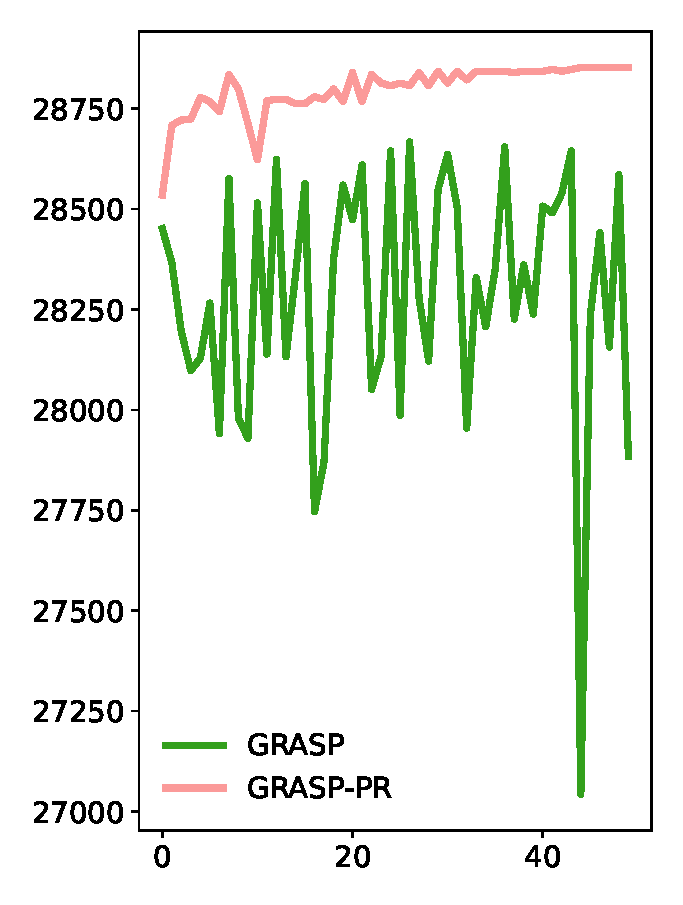
\includegraphics[scale=0.5]{knapPI_1_500_1000_1_iterations.eps}
	\caption{Execução da instância knapPI\_1\_500\_1000\_1}
\end{figure}

A primeira coisa que se percebe é que o GRASP-PR consegue manter a qualidade das soluções durante as execuções e chegando nas ultimas iterações ele aproximadamente converge em um ponto. Já o GRASP, como suas iterações são independentes, não apresenta essas características logo possui muito mais variações em execuções pois não é guiado por boas soluções anteriores.


\section{Conclusão}
\label{sec:orgdaf2bf9}
Uma adaptação da metaheurísticas Path Relinking foi proposta e combinada com o GRASP para solucionar o problema da mochila binária.

Foi possível observar com esse estudo que o GRASP com Path Relinking consegue guiar melhores soluções e também que a adição dessa método não adiciona significativamente em tempo computacional.
\end{document}